% https://www.overleaf.com/learn/latex/Beamer#Using_a_colorthemev

% Inbuilt themes in beamer
\documentclass[8pt, aspectratio=169, handout]{beamer}
% \documentclass[8pt, aspectratio=169]{beamer}

\input{../template/macros/macros_general.tex}
\input{../template/macros/macros_math.tex}
\input{../template/symbols/symbols_NN.tex}
\input{../template/symbols/symbols_robot.tex}

% ~~~~~~~~~~~~~~~~~~~~~~~~~~~~~~~~~~~~~~~~~~~~~~~~~~~~~~~~~~~~~~~~~~~~~~~~~~~~~~
% Block options: block, alertblock, exampleblock
% ~~~~~~~~~~~~~~~~~~~~~~~~~~~~~~~~~~~~~~~~~~~~~~~


% % Theme choice:
% \usetheme{Antibes}
% % \usecolortheme{beaver}
%~~~~~~~~~~~~~~~~~~~~~~~~~~~~~~~~~~~~~~~~~~~~~~~~~~~~~~~~~~~~~~~~~~~~~~~~~~~~~~
% Use roboto Font (recommended)
% \usepackage[sfdefault]{roboto}
\usepackage[utf8]{inputenc}
\usepackage[T1]{fontenc}
%~~~~~~~~~~~~~~~~~~~~~~~~~~~~~~~~~~~~~~~~~~~~~~~~~~~~~~~~~~~~~~~~~~~~~~~~~~~~~~

%~~~~~~~~~~~~~~~~~~~~~~~~~~~~~~~~~~~~~~~~~~~~~~~~~~~~~~~~~~~~~~~~~~~~~~~~~~~~~~
% Define where theme files are located. ('/styles')
\usepackage{styles/fluxmacros}
\usefolder{styles}
% Use Flux theme v0.1 beta
% Available style: asphalt, blue, red, green, gray 
\usetheme[style=blue]{flux}
%~~~~~~~~~~~~~~~~~~~~~~~~~~~~~~~~~~~~~~~~~~~~~~~~~~~~~~~~~~~~~~~~~~~~~~~~~~~~~~

%~~~~~~~~~~~~~~~~~~~~~~~~~~~~~~~~~~~~~~~~~~~~~~~~~~~~~~~~~~~~~~~~~~~~~~~~~~~~~~
% Extra packages for the demo:
\usepackage{booktabs}
\usepackage{colortbl}
\usepackage{ragged2e}
\usepackage{schemabloc}
%~~~~~~~~~~~~~~~~~~~~~~~~~~~~~~~~~~~~~~~~~~~~~~~~~~~~~~~~~~~~~~~~~~~~~~~~~~~~~~

\usepackage{multirow}
\usepackage{media9}

% Title page details: 
\title{
    Imposing a Weight Norm Constraint for Neuro-Adaptive Control 
} 
\subtitle{
    \textit{IEEE European Control Conference (ECC) 2025}\\
}
\author{
  \textbf{Myeongseok Ryu}\inst{1}, Jiyun Kim\inst{2}, and Kyunghwan Choi\inst{1}
  }
\date{2025-06-25}
\institute{%
    \begin{minipage}[c]{\linewidth}
        \centering
        \inst{1}%
        Department of Mechanical and Robotics Engineering\\
        Gwangju Institute of Science and Technology
        \and
        \inst{2}%
        AI Graduate School\\
        Gwangju Institute of Science and Technology
  \end{minipage}
}
\titlegraphic{assets/MIC_Lab_logo_white.png}
% make institute font size smaller
\setbeamerfont{institute}{size=\normalsize}

\AtBeginSection[]{%
  \frame<beamer>{ 
    \frametitle{Outline}   
    \tableofcontents[currentsection] 
  }
}

% \AtBeginSubsection[]{%
%   \begin{frame}
%   \vfill
%   \centering
%     \insertsectionhead
%     \\
%     \large\textbf{\insertsubsectionhead}
%   \vfill
%   \end{frame}
% }

\begin{document}

% Title page frame
\titlepage 

% Outline frame
\begin{frame}{Outline}
    \tableofcontents
\end{frame}

% ╔═══════════════════════════════════════════════╗
% ║ Section: Background and Contributions         ║
% ╚═══════════════════════════════════════════════╝
\section{Background and Contributions}

\subsection{Introduction to Neuro-Adaptive Control}

\begin{frame}{\insertsubsectionhead}{What is Neuro-Adaptive Control?}

  \textbf{Neuro-Adaptive Control}
  \small{
    \begin{itemize}
      \item \textbf{Neuro-adaptive control} (NAC) is a control strategy that combines \textbf{neural networks (NNs)} with \textbf{adaptive control} \cite{Farrell:2006aa}.
      \item Features of both \textbf{NNs} and \textbf{adaptive control} can be found in NAC.
    \end{itemize}
  }

  \begin{figure}
    \includegraphics[width=0.65\textwidth]{figures/NAC.drawio.pdf}
  \end{figure}

\end{frame} 


\begin{frame}{\insertsubsectionhead}{What is Neuro-Adaptive Control?}

  \textbf{Advantages of Neuro-Adaptive Control}
  \small{
    \begin{itemize}
      \item <+-> \textbf{Adaptability}: NAC adapts to changing environments and system dynamics.
      \item <+-> \textbf{Stability Guarantee}: The closed-loop stability is ensured using \textit{Lyapunov stability theory}.
      \item <+-> \textbf{Online Learning Capability}: NAC adapts in \textit{real-time} to new data with stability guarantees.
      \item <+-> \textbf{Robustness}: NAC handles \textit{uncertainties and disturbances} effectively with adaptive control techniques.
    \end{itemize}
  }
  
\begin{figure}
  \label{fig:general_framework}
  \includegraphics[width=0.65\textwidth]{figures/conv_nac.drawio.pdf}
  \caption{General framework of neuro-adaptive control (NAC).}
\end{figure}

\end{frame}

\begin{frame}{\insertsubsectionhead}{Existing Challenges in NAC}
  
  \begin{enumerate}
    \begin{columns}[T,onlytextwidth]
        \column{0.49\textwidth}
          \item \textbf{Weight Boundedness:}

          \begin{itemize}
            \item The NN weights can grow unbounded, leading to instability.
            \item Unbounded weights can cause the NN to produce large control inputs, which may lead to following challenges.
          \end{itemize}
          
        \column{0.49\textwidth}
          \centering
          \begin{figure}
            \includegraphics[width=0.4\textwidth]{figures/KAIST-hi.png}
            \caption{Unbounded NN weights.}
          \end{figure}
      \end{columns}

      \begin{columns}[T,onlytextwidth]
        \column{0.49\textwidth}
          \item \textbf{Unpredictable Amplitude of Control Input:}

          \begin{itemize}
            \item The NN outputs are unpredictable and not interpretable.
            \item This feature and unbounded NN weights can lead to control input saturation.
          \end{itemize}

        \column{0.49\textwidth}
          \centering
          \begin{figure}
            \includegraphics[width=0.8\textwidth]{figures/unpredictable.drawio.pdf}
            \caption{Unpredictable amplitude of NN outputs.}
          \end{figure}
      \end{columns}
  \end{enumerate}

\end{frame}

\subsection{Literature Review}

\begin{frame}{\insertsubsectionhead}
  
  \begin{enumerate}
    \begin{columns}[T,onlytextwidth]
        \column{0.65\textwidth}
          \item \textbf{Projection Operator} \small{\textit{for weight boundednss}}

          \begin{itemize}
            \item Projects the NN weights onto a convex set.
            \item Ensures that the weights remain within a predefined bound.
          \end{itemize}

          \begin{equation}
            \estwth \leftarrow \myproj_{\overline{\theta}}(\estwth)
          \end{equation}

        \column{0.35\textwidth}
          \begin{figure}
            \includegraphics[width=0.3\textwidth]{figures/KAIST-hi.png}
          \end{figure}
      \end{columns}

      \vspace{0.2cm}

      \begin{columns}[T,onlytextwidth]
        \column{0.65\textwidth}
          \item \textbf{$\epsilon$-modification, and $\sigma$-modification} \small{\textit{for weight boundednss}}

          \begin{itemize}
            \item Add a stabilizing term to adaptation law.
            \item Invariance set of the NN weights can be ensured.
          \end{itemize}

          \begin{equation}
            \ddtt{\estwth} \leftarrow \ddtt{\estwth} - \rho \norm{\estwth}
          \end{equation}

        \column{0.35\textwidth}
          \begin{figure}
            \includegraphics[width=0.3\textwidth]{figures/KAIST-hi.png}
          \end{figure}

      \end{columns}

      \vspace{0.2cm}

      \begin{columns}[T,onlytextwidth]
        \column{0.65\textwidth}
          \item \textbf{Additional Control Inputs} \small{\textit{for control saturation}}

          \begin{itemize}
            \item Conventional controllers are used to address control input saturation. 
                  \begin{itemize}
                    \item Barrier Lyapunov function or auxiliary system-based control inputs.
                  \end{itemize}
            \item These methods do not guarantee the stability of the system.     
          \end{itemize}

        \column{0.35\textwidth}

          \begin{figure}
            \includegraphics[width=0.3\textwidth]{figures/KAIST-hi.png}
          \end{figure}

      \end{columns}
  \end{enumerate}
\end{frame}

\begin{frame}{\insertsubsectionhead}{Limitations of Existing Methods}

  \textbf{Limitation 1: Lack of Optimality}
  \begin{itemize}
    \item The existing methods do not guarantee the optimality of the control input.
    \item ...
  \end{itemize}

  \textbf{Limitation 2: Disruption of Learning Process by Additional Control Inputs}
  \begin{itemize}
    \item Feedback tracking error for learning is disrupted by additional control inputs.
      \begin{itemize}
        \item The feedback error does not reflect the error induced by the NN, directly.
      \end{itemize}  
    \item 
  \end{itemize}

\end{frame}

\subsection{Contributions}

\begin{frame}{\insertsubsectionhead}

  \textbf{Contribution 1: Unified Optimization Framework} 
  \begin{itemize}
    \item 
  \end{itemize}

  \textbf{Contribution 2: Online Learning Capability (Stabiltiy Guarantees)}
  \begin{itemize}
    \item 
  \end{itemize}

  \textbf{Contribution 3: Weight and Control Input Constraint Handling}
  \begin{itemize}
    \item 
  \end{itemize}

\end{frame}

% ╔═══════════════════════════════════════════════╗
% ║ Section: Proposed Method                      ║
% ╚═══════════════════════════════════════════════╝
\section{Proposed Method}

\subsection{Architecture of the Proposed Method}

\begin{frame}{\insertsubsectionhead}
  
  \begin{columns}
    
    \column{0.5\textwidth}
      
      \textbf{Target Two-link Robotic Manipulator System}:
      \begin{itemize}
        \item Control input saturation function $\mysat(\cdot)$.
        \item Desired trajectory $\mv{q}_d$ is given.
      \end{itemize}
        \begin{equation}\label{eq:sys}
          \mm{M}\ddq + \mm{V}_m\dq + \mv{F} + \mv{G} + \mv{\tau}_d
          =
          \mysat(\mv{\tau})
        \end{equation}
      
      \textbf{Control Input}:
      \begin{itemize}
        \item NN's output $\mv{\Phi}$ is used as the control input.
        \item Consists of the estimated NN weights $\estwth$.
      \end{itemize}
      \begin{equation}\label{eq:input}
        \mv{\tau} := \mv{\Phi}(\mv{q}_n; \estwth)
      \end{equation}

      \textbf{Deep Neural Network (DNN)}:
      \begin{itemize}
        \item $k$ layers with $\estwth_i:=\myvec(\estwV_i)$.
        \item Activation function: $\phi(\cdot):=tanh(\cdot)$.
        \begin{equation}\label{eq:NN}
          \mv{\Phi}(\mv{q}_n; \estwth)
          :=
          \begin{cases}
              \estwV_i^\top \act_i(\estNN_{i-1}), 
              &
              i\in\{1,\dots ,k\},
              \\
              \estwV_0^\top {\q}_n,
              &
              i=0
              ,
          \end{cases}
        \end{equation}
      \end{itemize}

    \column{0.5\textwidth}  

      \begin{figure}
        \includegraphics[width=0.8\textwidth]{figures/Controller.drawio.pdf}
        \caption{Architecture of the proposed method.}
      \end{figure}

      \begin{figure}
        \includegraphics[width=0.7\textwidth]{figures/DNN.drawio.pdf}
        \caption{Architecture of the DNN.}
      \end{figure}

  \end{columns}

    \let\thefootnote\relax\footnote{
      \textit{Notations}: 
        $\mv{q}\in\R^n$: Joint position, $\mm{M}$: Inertia matrix, $\mm{C}$: Coriolis matrix, $\mm{G}$: Gravity vector, $\mv{\tau}$: Control input, $\estwth$: Estimated NN weights.
        $\estwth$: Estimated NN weights, $\mv{e}$: Tracking error, $\mv{\tau}_d$: Disturbance, $\mysat(\cdot)$: Saturation function.
      }

\end{frame}

\subsection{Problem Formulation}

\begin{frame}{\insertsubsectionhead}{Optimization Problem}

\begin{columns}

  \column{0.45\textwidth}

    \textbf{Optimization Problem Statement}:

    \begin{itemize}
      \item \textbf{Find} NN weights $\estwth$,
      \item That \textbf{minimize} objective function $J(\cdot)$,
        \begin{equation}\label{eq:obj}
          J(\mv{r};\estwth)
          := 
          \frac{1}{2} \mv{r}^\top \mv{r}.
        \end{equation}
        \begin{itemize}
          \item where $\mv{r} := \ddt\mv{e} + \Lambda\mv{e}$ is the filtered tracking error,
        \end{itemize}
      \item while satisfying the following \textbf{constraints}:
        \begin{itemize}
          \item Boundedness of the NN weights $\estwth$.
          \item Saturation of the control input $\mv{\tau}$.
        \end{itemize}
    \end{itemize}

  
  \column{0.5\textwidth}

    \begin{block}{Considered Constraints}

      \begin{itemize}
        \item \textbf{Weight Boundedness for Each Layer}: 
          \begin{equation}\label{eq:cstr:weight}
            c_{\theta_i}(\estwth)
            :=
            \norm{\estwth_i}^2 - \overline{\theta_i}^2 \le 0
            , 
            \forall i\in\{0,\ldots,k\}
          \end{equation}

        \item \textbf{Convex control Input Saturation}: 
          \begin{itemize}
            \item Input bound constraint:
            \begin{equation}\label{eq:cstr:input_bound}
              c_{\overline{\tau}_i}(\estwth)
              :=
              \tau_i - \overline{\tau_i}
              \le 
              0
              ,
              \quad
              c_{\underline{\tau}_i}(\estwth)
              :=
              \underline{\tau_i} - \tau_i
              \le 
              0
            \end{equation}
            \item Input norm constraint:
            \begin{equation}\label{eq:cstr:input_norm}
              c_{\mv{\tau}}(\estwth)
              :=
              \norm{\mv{\tau}}^2 - \overline{\tau}^2
              \le
              0
            \end{equation}
        \end{itemize}
      \end{itemize}
      
    \end{block}

  \end{columns}

  \let\thefootnote\relax\footnote{
    \textit{Notations}: 
    $\Lambda\in\R_{>0}^{n\times n}$: filtering matrix
  }

\end{frame}

\begin{frame}{\insertsubsectionhead}{Optimization Problem}

  \textbf{Original Optimization Problem}

  \begin{itemize}
    \item Constrained optimization problem to minimize the tracking error.
    \item Inequality constraints $c_j(\estwth) \le 0$ for $j\in\mathcal{I}$.
  \end{itemize}

    \begin{equation}\label{eq:opt_problem}
      \begin{matrix}
        \min_{\estwth} J(\mv{r};\estwth)
        \\\ \\
        \text{s.t. } c_{j}(\estwth) 
        \le 
        0
        ,
        \forall j\in\mathcal{I}
      \end{matrix}
    \end{equation}

  \textbf{Define Lagrangian Function}

  \begin{equation}\label{eq:lagrangian}
      L(\mv{r},\estwth,[\lambda_j]_{j\in\mathcal{I}})
      :=
      J(\mv{r};\estwth)
      +
      \sum_{j\in\mathcal{I}} \lambda_j c_j(\estwth)
  \end{equation}

  \textbf{Dual Problem}
  \begin{itemize}
    \item The dual problem is to minimize the Lagrangian function with respect to the NN weights $\estwth$, while maximizing the Lagrange multipliers $\lambda_j$.
    \item The Lagrange multipliers $\lambda_j$ are non-negative, \ie $\lambda_j \ge 0$.
  \end{itemize}

  \begin{equation}\label{eq:dual_problem}
    \min_{\estwth}\max_{[\lambda_j]_{j\in\mathcal{I}}} 
    L(\mv{r},\estwth,[\lambda_j]_{j\in\mathcal{I}})
  \end{equation}

\end{frame}

\subsection{Adaptation Law Derivation}

\begin{frame}{\insertsubsectionhead}{Gradient Descent/Ascent Method}
  
  To solve the dual problem, 
  \begin{equation}
    \min_{\estwth}\max_{[\lambda_j]_{j\in\mathcal{I}}} 
    L(\mv{r},\estwth,[\lambda_j]_{j\in\mathcal{I}})
    ,
  \end{equation}
  the first-order gradient descent/ascent method is used to derive the adaptation law.

  \centering
  \begin{minipage}{0.6\textwidth}%

    \begin{block}{Adaptation Law}%
      
    \textbf{Gradient Descent Method for $\estwth$}:
    \begin{equation}\label{eq:adaptation_law:1}
      \ddt {{\estwth}}
      =
      -\alpha 
      \ppfrac{L}{{\estwth}}
      =-\alpha 
      \left(
          \ppfrac{J}{{\estwth}}
          +
          \sum_{j\in\mathcal{I}}
          \lambda_j 
          \ppfrac{c_j}{\estwth}
      \right),
    \end{equation}

    \textbf{Gradient Ascent Method for $\lambda_j, \forall j\in\mathcal I$}:
    \begin{equation}\label{eq:adaptation_law:2}
      \ddt\lambda_j
      = 
      \beta_j
      \ppfrac{L}{\lambda_j} 
      = 
      \beta_j c_j ,
    \end{equation}

    For non-negativity of the Lagrange multipliers,
    \begin{equation}\label{eq:adaptation_law:3}
      \lambda_j
      \leftarrow
      \max(\lambda_j,0)
      .
    \end{equation}

    % \begin{subequations}
    %     \begin{align}
    %       \ddt {{\estwth}}
    %       &
    %       =
    %       -\alpha 
    %       \ppfrac{L}{{\estwth}}
    %       =-\alpha 
    %       \left(
    %           \ppfrac{J}{{\estwth}}
    %           +
    %           \sum_{j\in\mathcal{I}}
    %           \lambda_j 
    %           \ppfrac{c_j}{\estwth}
    %       \right),
    %       \\
    %       \ddt\lambda_j
    %       & 
    %       = 
    %       \beta_j
    %       \ppfrac{L}{\lambda_j} 
    %       = 
    %       \beta_j c_j ,
    %       \quad\quad\quad\quad      \      
    %       \forall j\in\mathcal I,
    %       \\
    %       \lambda_j
    %       &
    %       \leftarrow
    %       \max(\lambda_j,0)
    %     \end{align}
    % \end{subequations}

    \end{block}
  \end{minipage}
\end{frame}

\subsection{Stability Analysis}

\begin{frame}{\insertsubsectionhead}{Lyapunov Stability Analysis}

  \centering
  \begin{minipage}{.9\textwidth}

    \begin{block}{Theorem 1 \cite{Ryu:2025aa}}
      For the dynamical system described in \eqref{eq:sys}, the neuro-adaptive controller in \eqref{eq:input} with the weight adaptation laws in \eqref{eq:adaptation_law:1}, \eqref{eq:adaptation_law:2} and \eqref{eq:adaptation_law:3} ensure the boundedness of the filtered error $\mv{r}$ and the weight estimate $\estwth$, under the control input constraints satisfying Assumption 1 and 2. This holds under the weight norm constraint \eqref{eq:cstr:weight}.
    \end{block}

    \begin{exampleblock}{Assumption 1 (Convex Input Constraint)}
      The constraint functions $c_j(\estwth),\forall j\in\mathcal{I}$, are convex in the $\tau$-space and satisfy $c_j(\estwth)\le0$ and $c_j(\idealwth)\le0$.
    \end{exampleblock}

    \begin{exampleblock}{Assumption 2, Linear Independence Constraint Qualification (LICQ)}
      The selected constraints satisfy the Linear Independence Constraint Qualification (LICQ) \cite[Chap. 12 Def. 12.1]{Nocedal:2006aa}.
    \end{exampleblock}

  \end{minipage}

  \vspace{.2cm}

  Proof of Theorem 1 is omitted due to space limitations. The detailed proof can be found in \cite{Ryu:2025aa}.

\end{frame}

% ╔═══════════════════════════════════════════════╗
% ║ Section: Experimental Validation              ║
% ╚═══════════════════════════════════════════════╝
\section{Experimental Validation}

\subsection{Simulation Setup}

\begin{frame}{\insertsubsectionhead}{Two-Link Robotic Manipulator}

    \begin{columns}

      \column{.45\textwidth}

        \textbf{Target System}:

        \begin{equation*}
          \mm{M}\ddq + \mm{V}_m\dq + \mv{F} + \mv{G} + \mv{\tau}_d
          =
          \mv{\tau}
        \end{equation*}

        \begin{figure}
          \centering
          \includegraphics[width=.99\textwidth]{figures/RobotModel.drawio.png}
          \caption{Two-link robotic manipulator model.}
        \end{figure}

      \column{.55\textwidth}
      
        \textbf{Desired Trajectory}:

        \begin{equation}
          \qd
          =
          \begin{pmatrix}
              {q_d}_1\\
              {q_d}_2
          \end{pmatrix}
          = 
          \begin{pmatrix}
              +\cos(
                  \tfrac{\pi}{2}t
              ) + 1 \\
              -\cos(
                  \tfrac{\pi}{2}t
              ) - 1 
          \end{pmatrix}
          .
      \end{equation}

      \textbf{System Model Parameters}:

      \begin{table}
        \renewcommand{\arraystretch}{1.3}
        \caption{System model parameters.}
        \centering
        \begin{tabular}{c m{5em} c c c }
        \hline
        \textbf{Symbol} & \textbf{Description} & \textbf{Link 1} & \textbf{Link 2} \\
        \hline
        \hline 
        $m_p$ & Mass & 23.902 kg & 3.88 kg \\
        \hline
        $l_p$  & Length & 0.45 m & 0.45 m \\
        \hline
        ${l_c}_p$ & COM & 0.091 m & 0.048 m \\
        \hline
        $b_p$   & Viscous coef. &  2.288 Nms & 0.172 Nms \\
        \hline
        ${f_c}_p$  & Friction coef. & 7.17 Nm & 1.734 Nm \\
        \hline
        \end{tabular}
        \label{table: system parameters}
      \end{table}

    \end{columns}

\end{frame}

\begin{frame}{\insertsubsectionhead}{Controllers for Comparative Study}
  
    \begin{itemize}
      \item NAC-CO denotes the proposed controller based on constrained optimization.
      \item For NAC-L2 and NAC-eMod, the stabilizing terms $-\lambda\estwth$ and $\rho\norm{\tilde{\mv{z}}}\estwth$ ensures the boundedness of the NN weights
    \end{itemize}

    \begin{table}
      \renewcommand{\arraystretch}{1.5}
      % \caption{Controller Properties.}
      \centering
      \begin{tabular}{c m{20em} c c c }
      \hline
      \textbf{Name} & \textbf{Description} & \textbf{Adaptation Law} \\
      \hline
      \hline 
        \multirow{2}{*}{NAC-CO} & Constrained Optimization-based NAC & 
      $
        \ddt\estwth = -\alpha \left(\ppfrac{L}{\estwth}+\sum_{j\in\mathcal{I}}\lambda_j\ppfrac{c_j}{\estwth}\right)
      $ 
      \\
        (proposed) & ($\beta_j$ determines $\lambda_j$ adaptation speed) &
      $
        \ddt\lambda_j = \beta_j c_j, \lambda_j \leftarrow \max(\lambda_j,0)
      $
      \\
      \hline
      \multirow{2}{*}{NAC-L2} & NAC with $L_2$-regularization & \multirow{2}{*}
      {$
        \ddt\estwth = -\alpha \left(\ppfrac{J}{\estwth}+\lambda\estwth\right)
      $}
      \\
        & ($\lambda\in\R_{>0}$ stabilizes $\estwth$ towards origin) &
      \\
      \hline
      \multirow{2}{*}{NAC-eMod} & NAC with $\epsilon$-modification & \multirow{2}{*}
      {$
        \ddt\estwth = -\alpha \left(\ppfrac{J}{\estwth}+\rho\norm{\tilde{\mv{z}}}\estwth\right)
      $}
      \\
      & ($\rho$ stabilizes proportionally to the error $\tilde{\mv{z}}$) &
      \\
      \hline
      \end{tabular}
      \label{table:sys:param}
    \end{table}

    \centering
    \begin{minipage}{0.75\textwidth}
      \begin{block}{Simulation Objective}
        By varying the parameters, \ie $\beta_j$, $\lambda$, and $\rho$, the parameter dependencies will be investigated.
      \end{block}
    \end{minipage}

\end{frame}

\subsection{Simulation Results}

\begin{frame}{\insertsubsectionhead}{Box-and-Whisker Plots}
  
  \begin{columns}
    \column{0.55\textwidth}
    
      \textbf{Parameter Dependencies Investigation}:

      \begin{itemize}
        \item The parameters ranged from 0.001 to 1 across 10 samples.
        \item NAC-CO (proposed) shows the best performance and low variance.
        \item NAC-L2 shows the worst performance with high variance.
      \end{itemize}

    \column{0.5\textwidth}

      \begin{figure}
        \includegraphics[width=.99\textwidth]{figures/BoxWhisker.drawio.png}
        \caption{Parameter dependencies of the proposed method.}
      \end{figure}

  \end{columns}

    \begin{table}[!t]
      \renewcommand{\arraystretch}{1.1}
      % \caption{Quantitative comparison of square root of tracking ISE.}
      \centering
      \begin{tabular}{c c c c }
      \hline
      & \textbf{NAC-L2}\!&\!\textbf{NAC-eMod}\!&\!\textbf{NAC-CO} (proposed) 
      \\
      \hline
      \hline 
        Maximum\!&\!$11.1753\!\times\!10^{-3}$\!&\!$0.5603\!\times\!10^{-3}$\!&\!$0.3439\!\times\!10^{-3}$\!\\
      \hline
        Median\!&\!$0.5898\!\times\!10^{-3}$\!&\!$0.5519\!\times\!10^{-3}$\!&\!$0.3240\!\times\!10^{-3}$\!\\
      \hline
        Minimum\!&\!$0.5434\!\times\!10^{-3}$\!&\!$0.5434\!\times\!10^{-3}$\!&\!$0.3235\!\times\!10^{-3}$\!\\
      \hline
      \end{tabular}
      \label{table: error norm}
    \end{table}
    
    \let\thefootnote\relax\footnote{
      Squared root of the tracking error ISE (Integral of Squared Error) is used, \ie $\sqrt{\int_0^T \norm{\mv{r}}^2\,\der t}$, where $T$ denotes a simulation termination time.
    }
    
\end{frame}

\begin{frame}{\insertsubsectionhead}{Weight Norms}

  \begin{columns}

    \column{0.33\textwidth}

      \begin{figure}
        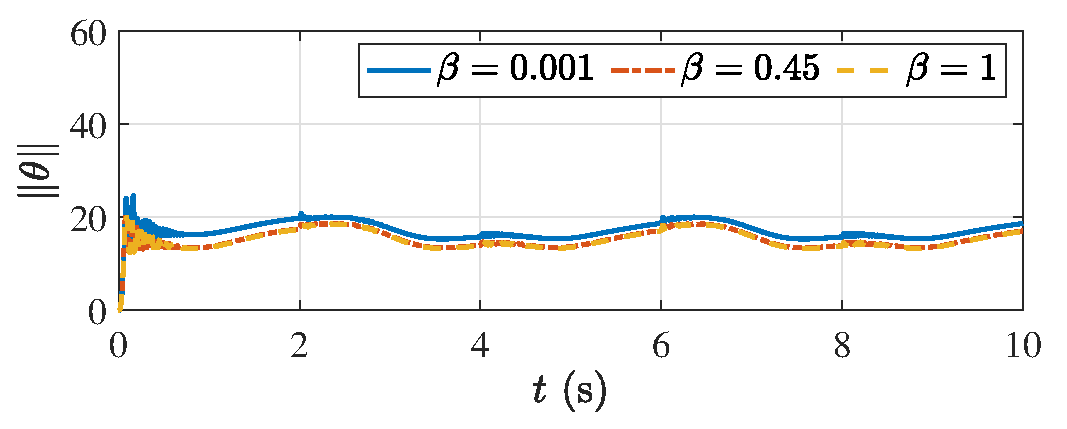
\includegraphics[width=0.99\textwidth]{figures/ECC/fig8.eps}
        \caption{Weight norms of NAC-CO}
      \end{figure}

    \column{0.33\textwidth}

      \begin{figure}      
        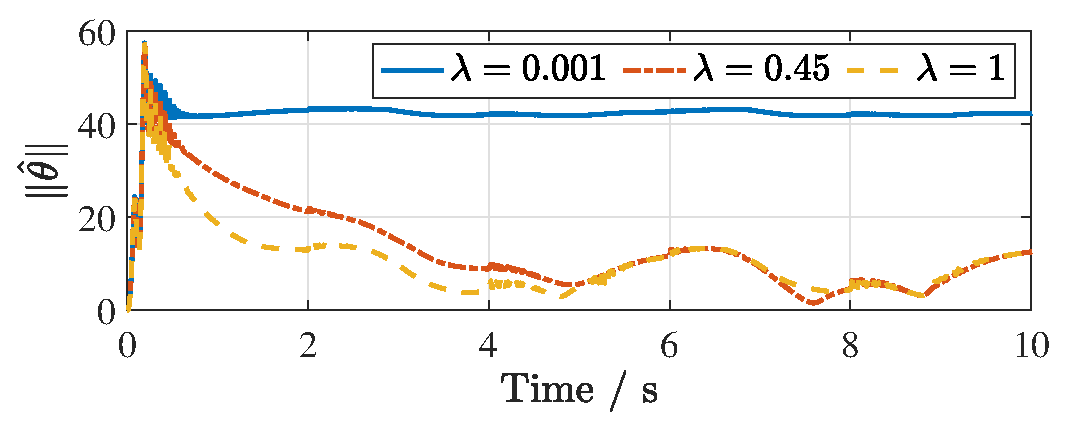
\includegraphics[width=0.99\textwidth]{figures/ECC/fig9.eps}
        \caption{Weight norms of NAC-L2}
      \end{figure}
      
    \column{0.33\textwidth}

      \begin{figure}
        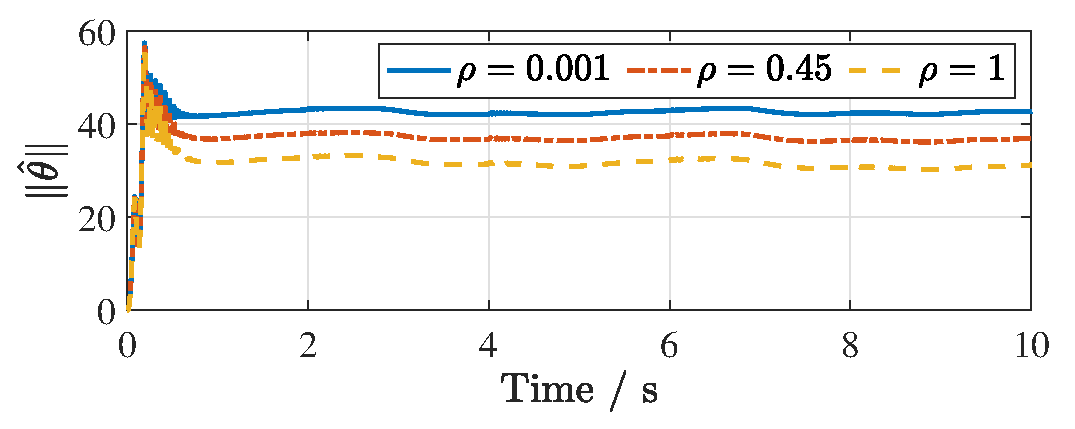
\includegraphics[width=0.99\textwidth]{figures/ECC/fig10.eps}
        \caption{Weight norms of NAC-eMod}
      \end{figure}
    
  \end{columns}

  \begin{itemize}
    \item NAC-CO (proposed) showed the weight norms are bounded under pre-defined constraint $\overline{\theta}=20$.
    \item NAC-L2 and NAC-eMod showed the bounded weight norms, but they depended on the parameters $\lambda$ and $\rho$, respectively.
    \item As the parameters $\lambda$ and $\rho$ increase, the weight norms of NAC-L2 and NAC-eMod biased towards the origin, which may lead to suboptimal performance.
    \item In addition, NAC-CO tracked the desired trajectory with a smaller weight norm than NAC-L2 and NAC-eMod.
  \end{itemize}

\end{frame}

\begin{frame}{\insertsubsectionhead}{Tracking Performance}

  \begin{columns}

    \column{0.33\textwidth}

      \begin{figure}
        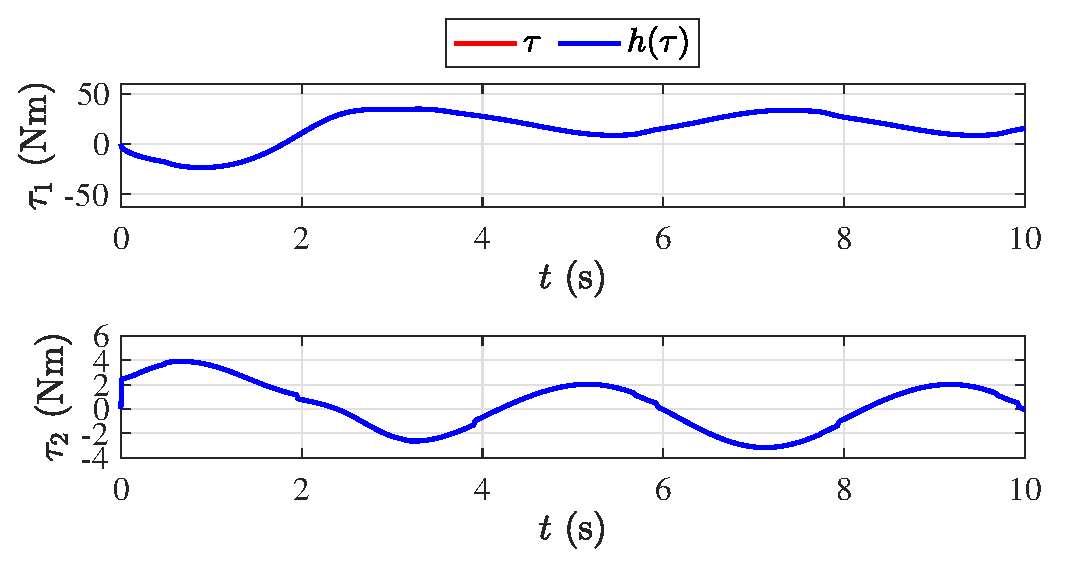
\includegraphics[width=0.99\textwidth]{figures/ECC/fig5.eps}
        \caption{Tracking error of NAC-CO}
      \end{figure}
    
    \column{0.33\textwidth}

      \begin{figure}      
        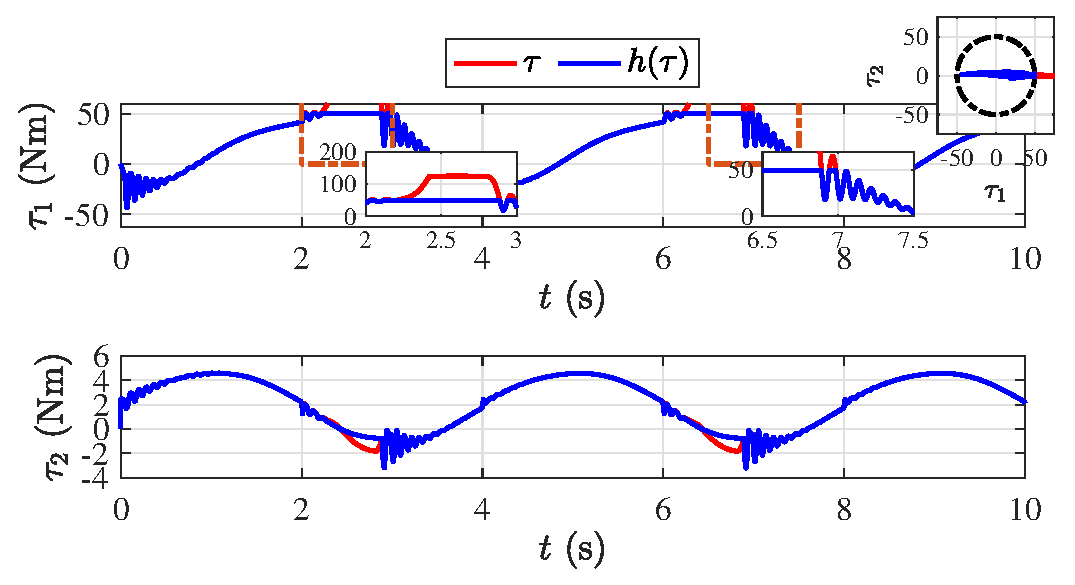
\includegraphics[width=0.99\textwidth]{figures/ECC/fig6.eps}
        \caption{Tracking error of NAC-L2}
      \end{figure}
      
    \column{0.33\textwidth}

      \begin{figure}
        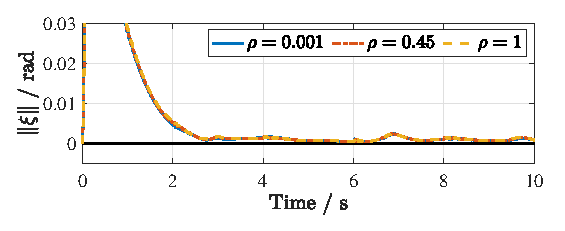
\includegraphics[width=0.99\textwidth]{figures/ECC/fig7.eps}
        \caption{Tracking error of NAC-eMod}
      \end{figure}

  \end{columns}

  \begin{itemize}
    \item NAC-CO (proposed) outperformed NAC-L2 and NAC-eMod in terms of tracking performance.
    \item As the weights are biased towards the origin, the tracking performance of NAC-L2 and NAC-eMod deteriorated.
  \end{itemize}

\end{frame}

% \begin{frame}{Representative Simulation Results}

%   \centering
%   \includemedia[
%       width=0.96\linewidth,
%       height=0.54\linewidth,
%       activate=onclick,
%       addresource=demonstration.mp4,
%       flashvars={
%          source=demonstration.mp4
%         &autoPlay=true
%         &loop=true
%       }
%     ]{}{VPlayer.swf}

% \end{frame}

% \subsection{Simulation Setup}

% \begin{frame}{\insertsubsectionhead}{Two-Link Robotic Manipulator}

%     \begin{columns}

%       \column{.55\textwidth}
%         \begin{figure}
%           \centering
%           \includegraphics[width=.85\textwidth]{figures/RobotModel.drawio.png}
%           \caption{Two-Link Robotic Manipulator}
%         \end{figure}

%       \column{.5\textwidth}
      
%         \begin{table}[t]
%             \renewcommand{\arraystretch}{1.3}
%             \caption{Two-link robotic manipulator's parameters.}
%             \centering
%             \begin{tabular}{c m{9.5em} c c c }
%             % \begin{tabular}{c c c c c}
%             \hline
%             \textbf{Symbol} & \textbf{Description} & \textbf{Value} \\
%             \hline
%             \hline 
%             $m_1,m_2$ & Mass & 2.465 kg \\
%             \hline
%             $l_1,l_2$  & Length & 0.2 m \\  
%             \hline
%             ${l_c}_1,{l_c}_2$ & Center of mass & 0.139 m \\
%             \hline
%             $I_1,I_2$  & Inertia & 0.069 kgm\textsuperscript{2} \\
%             \hline
%             \end{tabular}
%         \end{table}

%     \end{columns}

% \end{frame}

% ╔═══════════════════════════════════════════════╗ 
% ║ Section: Conclusion and Future Work           ║
% ╚═══════════════════════════════════════════════╝
\section{Conclusion}

\subsection{Conclusion and Future Work}

\begin{frame}{Conclusion}
    
  \textbf{Summary of Contributions}
  \begin{itemize}
    \item Proposed a novel constrained optimization-based neuro-adaptive control (CONAC) method.
    \item Adaptation laws are derived using constrained optimization method.
    \item The proposed method guarantees the stability of the system and the boundedness of the NN weights.
    \item Feasibility of the proposed method is validated through numerical simulations and real-time experiments.
  \end{itemize}

  \textbf{Future Work}
  \begin{itemize}
    \item Extend the proposed method to state constraints.
    \item Enhance the robustness and flexibility of the proposed method for various systems.
  \end{itemize}

\end{frame}

\section{}
\begin{frame}{}
    \centering \Large
    \emph{Thank you for your attention!}
\end{frame}

\begin{frame}[allowframebreaks]{References}

  \bibliography{localRefs}
  \bibliographystyle{IEEEtran}

\end{frame}

\end{document}